% Created 2016-08-10 Wed 20:54
\documentclass[presentation]{beamer}
\usepackage[utf8]{inputenc}
\usepackage[T1]{fontenc}
\usepackage{fixltx2e}
\usepackage{graphicx}
\usepackage{grffile}
\usepackage{longtable}
\usepackage{wrapfig}
\usepackage{rotating}
\usepackage[normalem]{ulem}
\usepackage{amsmath}
\usepackage{textcomp}
\usepackage{amssymb}
\usepackage{capt-of}
\usepackage{hyperref}
\author{Nasser Alkmim}
\date{\today}
\title{Curso de Python - 2 dia}
\hypersetup{
 pdfauthor={Nasser Alkmim},
 pdftitle={Curso de Python - 2 dia},
 pdfkeywords={},
 pdfsubject={},
 pdfcreator={Emacs 24.5.1 (Org mode 8.3.5)}, 
 pdflang={English}}
\begin{document}

\maketitle

\section{Introdução}
\label{sec:orgheadline4}
\subsection{Ementa}
\label{sec:orgheadline1}
Nesse módulo serão tratados os seguintes assuntos:

\begin{enumerate}
\item Numpy
\item Matplotlib
\item OOP
\end{enumerate}
\subsection{Motivação rápida}
\label{sec:orgheadline2}


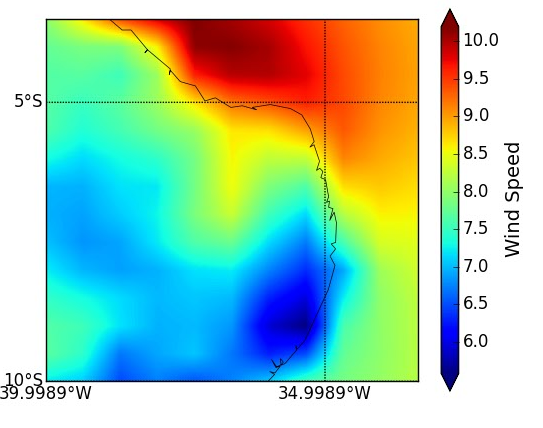
\includegraphics[width=.9\linewidth]{img/msa-presentation.org_20160406_222911_.png}
\subsection{Motivação rápida}
\label{sec:orgheadline3}


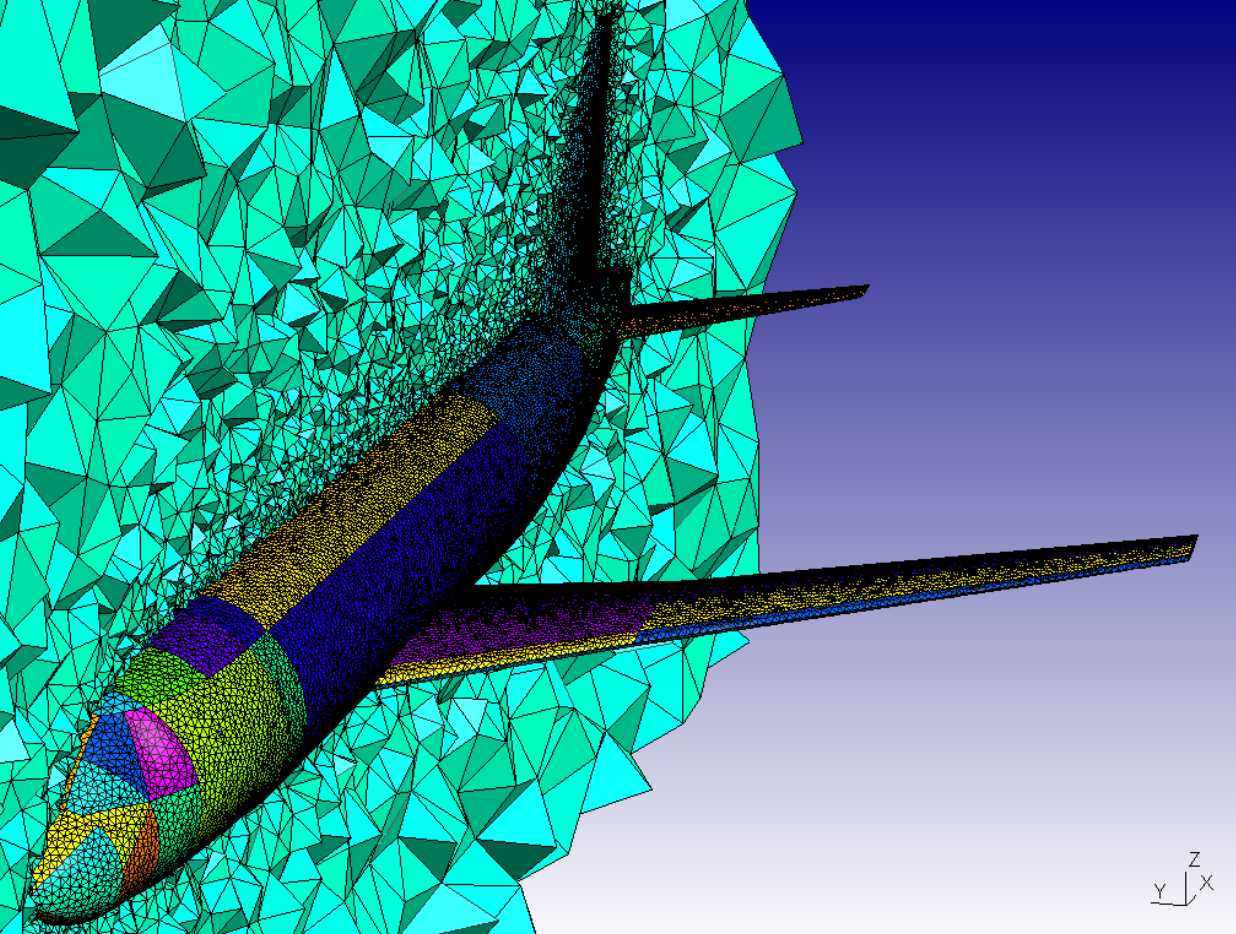
\includegraphics[width=.9\linewidth]{img/Introdução/Capture_2016-08-10_14-57-31.PNG}

\section{Numpy}
\label{sec:orgheadline26}
\subsection{O que é numpy?}
\label{sec:orgheadline5}

\begin{enumerate}
\item Biblioteca para computação científica em Python.
\item Um equivalente ao Matlab
\item Operações matriciais/vetoriais
\item Kit para álgebra linear
\end{enumerate}

\subsection{Como usar}
\label{sec:orgheadline6}

\begin{enumerate}
\item Baixar a biblioteca
\end{enumerate}

\begin{verbatim}
pip install numpy
\end{verbatim}

\begin{verbatim}
conda install numpy
\end{verbatim}

\begin{enumerate}
\item Importar a biblioteca
\end{enumerate}

\begin{verbatim}
import numpy as np
\end{verbatim}

\subsection{Criação de arrays}
\label{sec:orgheadline7}

Arrays em 1D não são linha nem coluna
\begin{verbatim}
import numpy as np
vetor = np.array([1, 2, 3, 5])

print(vetor, vetor.T)
\end{verbatim}

\begin{verbatim}
[1 2 3 5] [1 2 3 5]
\end{verbatim}

\begin{verbatim}
matriz = np.array([[1, 2, 3],
                   [4, 5, 6]])
print(matriz)
\end{verbatim}

\begin{verbatim}
[[1 2 3]
 [4 5 6]]
\end{verbatim}


\subsection{Convertendo lista para arrays}
\label{sec:orgheadline8}

\begin{verbatim}
a = [[1, 2, 3], [10, 22, 33]]
A = np.array(a)

print('1 \n', a)
print('2 \n', A)
print('3 \n', a[1][2])
print('4 \n', A[1, 2])
\end{verbatim}

\begin{verbatim}
1 
 [[1, 2, 3], [10, 22, 33]]
2 
 [[ 1  2  3]
 [10 22 33]]
3 
 33
4 
 33
\end{verbatim}

\subsection{Iniciando arrays}
\label{sec:orgheadline9}

\begin{verbatim}
zero = np.zeros(5)
print(zero)

m_zeros = np.zeros((3,3))
print(m_zeros)
\end{verbatim}

\begin{verbatim}
[ 0.  0.  0.  0.  0.]
[[ 0.  0.  0.]
 [ 0.  0.  0.]
 [ 0.  0.  0.]]
\end{verbatim}
\subsection{Slicing de arrays 1D}
\label{sec:orgheadline10}

\begin{verbatim}
A = np.linspace(0, 10, 11)
print('1', A)
print('2', A[:])
print('3', A[...])
print('4', A[5:7])
print('5', A[5:])
print('6', A[::2])
\end{verbatim}

\begin{verbatim}
1 [  0.   1.   2.   3.   4.   5.   6.   7.   8.   9.  10.]
2 [  0.   1.   2.   3.   4.   5.   6.   7.   8.   9.  10.]
3 [  0.   1.   2.   3.   4.   5.   6.   7.   8.   9.  10.]
4 [ 5.  6.]
5 [  5.   6.   7.   8.   9.  10.]
6 [  0.   2.   4.   6.   8.  10.]
\end{verbatim}

\subsection{Slicing de arrays 2D}
\label{sec:orgheadline11}

\begin{verbatim}
np.set_printoptions(precision=1)
A = np.random.rand(5, 3)
print('1 \n', A)
print('2 \n', A[:, ...])
print('3 \n', A[:, 0])
print('4 \n', A[0, :])
\end{verbatim}

\begin{verbatim}
1 
 [[ 0.9  0.7  0.7]
 [ 0.7  0.3  0.8]
 [ 0.8  0.2  0.2]
 [ 0.1  0.3  0.1]
 [ 0.9  0.4  0.5]]
2 
 [[ 0.9  0.7  0.7]
 [ 0.7  0.3  0.8]
 [ 0.8  0.2  0.2]
 [ 0.1  0.3  0.1]
 [ 0.9  0.4  0.5]]
3 
 [ 0.9  0.7  0.8  0.1  0.9]
4 
 [ 0.9  0.7  0.7]
\end{verbatim}





\subsection{Operações com matrizes}
\label{sec:orgheadline12}

\begin{verbatim}
A = np.array([[1, 2, 3], [4, 5, 6]])
B = np.array([8, 9, 10])
c = 100
print(A, B, '\n')
print(np.shape(A), np.shape(B), '\n')
print(A*c, '\n')
print(A @ B) # Python 3.5
print(np.dot(A, B))
\end{verbatim}

\begin{verbatim}
[[1 2 3]
 [4 5 6]] [ 8  9 10] 

(2, 3) (3,) 

[[100 200 300]
 [400 500 600]] 

[ 56 137]
[ 56 137]
\end{verbatim}

\subsection{Solução de sistemas lineares}
\label{sec:orgheadline13}


\begin{verbatim}
A = np.array([[1, 2, 3], [4, 5, 6], [2, 5, 6]])
B = np.array([8, 9, 10])

# Solve Ax=B
x = np.linalg.solve(A, B)

print(A, B)
print(x)
\end{verbatim}

\begin{verbatim}
[[1 2 3]
 [4 5 6]
 [2 5 6]] [ 8  9 10]
[-0.5        -6.          6.83333333]
\end{verbatim}
\subsection{Produto interno}
\label{sec:orgheadline14}

\begin{verbatim}
a = [1, 2, 3, 4, 5]
b = [3, 4, 5, 6, 7]

sum = 0
for i in range(len(a)):
    sum = sum + a[i] * b[i]
print(sum)
\end{verbatim}

\begin{verbatim}
85
\end{verbatim}
\subsection{Produto interno pythonic}
\label{sec:orgheadline15}

\begin{verbatim}
a = [1, 2, 3, 4, 5]
b = [3, 4, 5, 6, 7]

sum = 0
for x, y in zip(a, b):          # unpacking os membros da lista
    sum += x*y
print(sum)
\end{verbatim}

\begin{verbatim}
85
\end{verbatim}
\subsection{Produto interno numpy}
\label{sec:orgheadline16}

\begin{verbatim}
import numpy as np
a = np.array([1, 2, 3, 4, 5])
b = np.array([3, 4, 5, 6, 7])

print(np.sum(a*b))
\end{verbatim}

\begin{verbatim}
85
\end{verbatim}
\subsection{Produto interno álgebra linear}
\label{sec:orgheadline17}

\begin{verbatim}
import numpy as np
a = np.array([1, 2, 3, 4, 5])
b = np.array([3, 4, 5, 6, 7])

print(a @ b)
print(np.dot(a, b))
\end{verbatim}

\begin{verbatim}
85
85
\end{verbatim}

\subsection{Polinômios}
\label{sec:orgheadline18}

\begin{verbatim}
import numpy as np

print(np.roots([2, 0, -1]))     # p[0] * x**n + p[1] * x**(n-1) + ... + p[n-1]*x + p[n]

p = np.poly1d([1, 0, 1])        # definir um polinômio em uma variável
print(p, '\n', np.roots(p), np.roots([1, 0, 1]))
\end{verbatim}

\begin{verbatim}
[-0.70710678  0.70710678]
   2
1 x + 1 
 [-0.+1.j  0.-1.j] [-0.+1.j  0.-1.j]
\end{verbatim}

\subsection{Diferenças finitas}
\label{sec:orgheadline19}


\begin{verbatim}
import numpy as np

x = np.linspace(0.78, 0.79, 100)
y = np.sin(x)
dy_analy = np.cos(x)

dy_numer = [0.0]*len(x)
# print(dy_numer)
for i in range(len(y) - 1):
    dy_numer[i] = (y[i+1] - y[i])/(x[i+1] - x[i])
dy_numer[-1] = (y[-1] - y[-2])/(x[-1] - x[-2])  # o ultimo termo
\end{verbatim}

\subsection{Comparação}
\label{sec:orgheadline20}

\begin{verbatim}
%matplotlib inline
import matplotlib.pyplot as plt

plt.plot(x, dy_analy, '-r', label='analytical')
plt.plot(x, dy_numer, '-b', label='forward')
plt.legend(loc='lower left')
\end{verbatim}

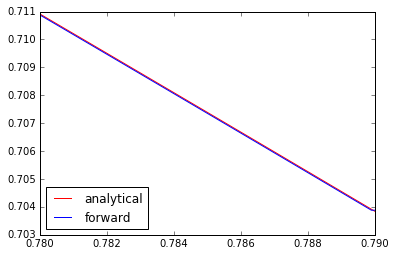
\includegraphics[width=.9\linewidth]{img/diffin.png}
\subsection{Integral}
\label{sec:orgheadline21}

\begin{verbatim}
import numpy as np

x = np.array([0, 0.5, 1, 1.5, 2])  # Conjunto de dados com 5 pontos
y = x**3                        # integral x4/4 0 a 2 = 4

integral = np.trapz(y, x)

error = (integral - 4)/4        # divide por 4 intervalos

print(integral, error)
\end{verbatim}

\begin{verbatim}
4.25 0.0625
\end{verbatim}
\subsection{Integral}
\label{sec:orgheadline22}

\begin{verbatim}
%matplotlib inline
import numpy as np
import matplotlib.pyplot as plt

x = np.array([0, 0.5, 1, 1.5, 2])
y = x**3

x2 = np.linspace(0, 2, 50)
y2 = x2**3

plt.plot(x, y, label='5 pontos')
plt.plot(x2, y2, label='50 pontos')
plt.legend()
\end{verbatim}

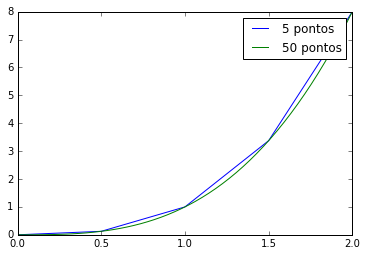
\includegraphics[width=.9\linewidth]{img/int.png}
\subsection{Problema}
\label{sec:orgheadline23}

\begin{verbatim}
M = np.zeros((3,3))
print(M)
gl = [0, 2]

m = np.array([[10, 11], [12, 13]])
print(m)
\end{verbatim}

\begin{verbatim}
[[ 0.  0.  0.]
 [ 0.  0.  0.]
 [ 0.  0.  0.]]
[[10 11]
 [12 13]]
\end{verbatim}
\subsection{Problema solução bruta}
\label{sec:orgheadline24}

\begin{verbatim}
M = np.zeros((3,3))
gl = [0, 2]
m = np.array([[10, 11], [12, 13]])

for i in range(len(gl)):        # loop em 0 e 1
    for j in range(len(gl)):    # loop em 0 e 1
        M[gl[i], gl[j]] = m[i, j]

print(M)
\end{verbatim}

\begin{verbatim}
[[ 10.   0.  11.]
 [  0.   0.   0.]
 [ 12.   0.  13.]]
\end{verbatim}

\subsection{Problema pythonic}
\label{sec:orgheadline25}

\begin{verbatim}
M = np.zeros((3,3))
gl = [0, 2]
m = np.array([[10, 11], [12, 13]])

id = np.ix_(gl, gl)             # array (2, 1) e (1, 2)
print(id)

M[id] = m
print(M)
\end{verbatim}

\begin{verbatim}
(array([[0],
       [2]]), array([[0, 2]]))
[[ 10.   0.  11.]
 [  0.   0.   0.]
 [ 12.   0.  13.]]
\end{verbatim}


\section{Matplotlib}
\label{sec:orgheadline41}
\subsection{O que é?}
\label{sec:orgheadline27}

\begin{enumerate}
\item Biblioteca para plotar gráficos 2D (principalmete)
\item Pode ser usada de duas maneiras
\begin{enumerate}
\item Pyplot --> módulo equivalente ao Matlab
\item OOP --> "pythonic way"
\end{enumerate}
\end{enumerate}

\subsection{Pyplot interface --> Matlab equilavente}
\label{sec:orgheadline28}

\begin{verbatim}
%matplotlib inline
import numpy as np
import matplotlib.pyplot as plt

x = np.linspace(0, 2*np.pi, 50)
y = np.sin(x)
plt.plot(x, y, '-b', linewidth=10, color='yellow')            # Cria Figure e Axes

# Configurações
plt.xlabel('x Axis')            # Usa o Axes atual
plt.ylabel('y Axis')
plt.title('Plot de uma Senoide')
plt.xlim(0, 2*np.pi)
plt.ylim(-1, 1)
plt.legend([r'$\sin(x)$'])          # lista de strings
\end{verbatim}

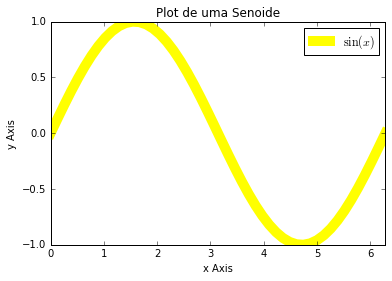
\includegraphics[width=.9\linewidth]{img/plt1.png}
\subsection{Exercício}
\label{sec:orgheadline29}

\textbf{Plotar a função}

\(f(x) = 3  \cos(5x + \pi/2) + \cos(4pi/5)\)

\subsection{Exercício solução}
\label{sec:orgheadline30}

\begin{verbatim}
%matplotlib inline
import numpy as np
import matplotlib.pyplot as plt

x = np.linspace(0, 2*np.pi, 100)
y = 3*np.cos(5*x + np.pi/2) + np.cos(4*np.pi/5)
plt.plot(x, y, '-r')            # Cria Figure e Axes

# Configurações
plt.xlabel('x Axis')            # Usa o Axes atual
plt.ylabel('y Axis')
plt.title('Plot do Exercício')
plt.xlim(0, 2*np.pi)
# plt.ylim(-2, 2)
plt.legend([r'$Exercício$'])          # lista de strings
\end{verbatim}

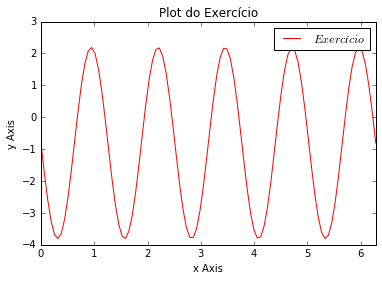
\includegraphics[width=.9\linewidth]{img/pltcos.png}


\subsection{Plot de Iso-linhas usando o módulo Pyplot}
\label{sec:orgheadline31}

\begin{verbatim}
%matplotlib inline
import numpy as np
import matplotlib.pyplot as plt

x = np.linspace(0, 10, 20)      # 1D array
y = np.linspace(0, 10 ,20)      # 1D array
X, Y = np.meshgrid(x, y)        # 2D array
Z = np.sin(X)**2 + np.sin(Y)**2 # Valor em cada ponto do plano (x,y)

plt.contour(X, Y, Z)

# Configurações
plt.xlabel('x Axis')
plt.ylabel('y Axis')
plt.title('Plot')
\end{verbatim}

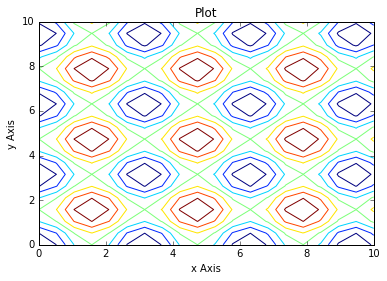
\includegraphics[width=.9\linewidth]{img/plt_2.png}


\subsection{Conceitos gerais matplotlib OOP API}
\label{sec:orgheadline32}

\begin{enumerate}
\item Hierarquia
\end{enumerate}

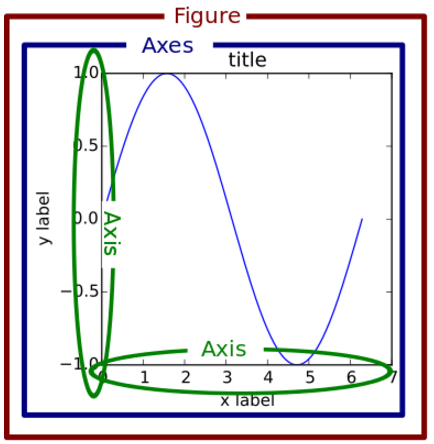
\includegraphics[width=.9\linewidth]{img/curso-python-dia-2.org_20160804_085108_.png}

\subsection{Criar Figure e Axes}
\label{sec:orgheadline33}


\begin{verbatim}
%matplotlib inline
import numpy as np
import matplotlib.pyplot as plt  # Usa o pyploy para criar o obj Figure apenas!

fig = plt.figure()              # cria o objeto: Figure
ax = fig.add_axes([0.1, 0.1, 0.8, 0.8]) # cria o objeto: Axes, filho da Figure
fig.show()
\end{verbatim}

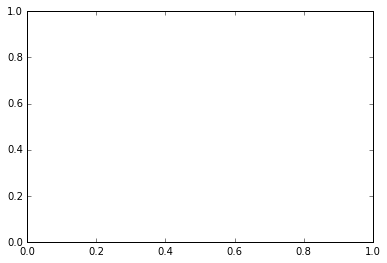
\includegraphics[width=.9\linewidth]{img/plt_3.png}
\subsection{Figure contém os Axes filhos}
\label{sec:orgheadline34}


\begin{verbatim}
%matplotlib inline
import numpy as np
import matplotlib.pyplot as plt

fig = plt.figure()              
ax1 = fig.add_axes([0.1, 0.1, 0.3, 0.3]) 
ax2 = fig.add_axes([0.5, 0.5, 0.3, 0.3])
fig.show()
\end{verbatim}

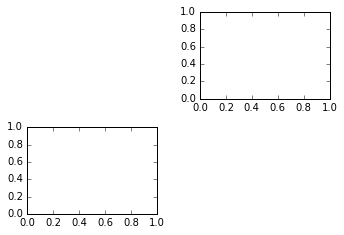
\includegraphics[width=.9\linewidth]{img/plt_4.png}


\subsection{E onde vejo os dados?}
\label{sec:orgheadline35}

\begin{enumerate}
\item Tudo que se vê dentro de um gráfico é chamado de \textbf{Artist}
\item Os \textbf{Artist} são criados por \emph{métodos} do \emph{objeto} \textbf{Axes}
\end{enumerate}


\subsection{Criando Artists}
\label{sec:orgheadline36}

\begin{verbatim}
%matplotlib inline
import numpy as np
import matplotlib.pyplot as plt

x = np.linspace(0, 10, 50)
y = np.sin(x)

fig = plt.figure()
ax = fig.add_axes([.1, .1, .8, .8]) # [lc, bc, wi, he]

ax.plot(x, y, '-r')             # método do objeto Axes

# Configurações 
ax.set_xlabel(r'$x$')
ax.set_ylabel(r'$y$')
\end{verbatim}

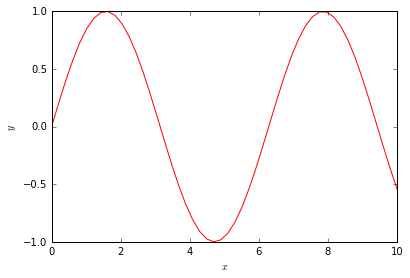
\includegraphics[width=.9\linewidth]{img/plt_5.png}
\subsection{Vantagem da abordagem OOP}
\label{sec:orgheadline37}

\begin{verbatim}
%matplotlib inline
import numpy as np
import matplotlib.pyplot as plt

x = np.linspace(0, 10, 50)
y = np.sin(x)

fig = plt.figure()              # Pyplot para criar Figure
ax1 = fig.add_axes([.1, .1, .8, .8])
ax2 = fig.add_axes([.2, .55, .3, .3])

ax1.plot(x, y, '-r')
ax2.plot(x, y, '-b')

ax2.set_xlim(0, 1)              # Um detalhe
\end{verbatim}

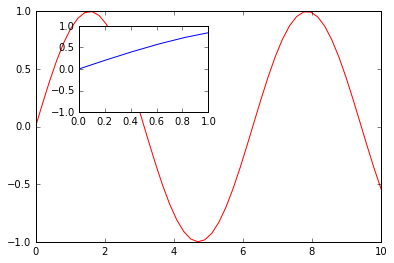
\includegraphics[width=.9\linewidth]{img/plt_6.png}
\subsection{3 Dimensões - 2D arrays}
\label{sec:orgheadline38}

\begin{verbatim}
%matplotlib inline
import numpy as np
import matplotlib.pyplot as plt
from mpl_toolkits.mplot3d import Axes3D

x = np.linspace(0, 1)
y = np.linspace(-2, 1)

X, Y = np.meshgrid(x, y)        # 2D arrays
Z = (X - 3)**2 + (Y + 1)**2     # Função do espaço (x, y)

fig = plt.figure()
ax = Axes3D(fig)
ax.plot_surface(X, Y, Z, cmap='viridis')  # Cira superfície
\end{verbatim}

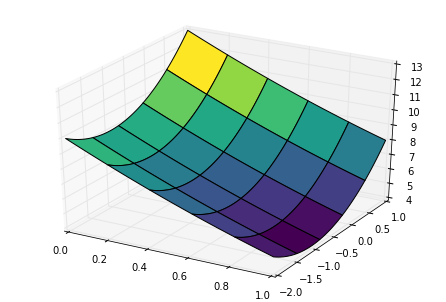
\includegraphics[width=.9\linewidth]{img/plt_7.png}


\subsection{3 Dimensões Exemplo - 1D arrays}
\label{sec:orgheadline39}

\begin{verbatim}
%matplotlib inline
import numpy as np
import matplotlib.pyplot as plt
from mpl_toolkits.mplot3d import Axes3D

n_angles = 36
n_radii = 8

radii = np.linspace(0.125, 1.0, n_radii)  # raios
angles = np.linspace(0, 2*np.pi, n_angles, endpoint=False)  # ângulos

angles = np.repeat(angles[..., np.newaxis], n_radii, axis=1)

x = np.append(0, (radii*np.cos(angles)).flatten())
y = np.append(0, (radii*np.sin(angles)).flatten())

z = np.sin(-x*y)                # multiplicação termo a termo

fig = plt.figure()
ax = Axes3D(fig)
ax.plot_trisurf(x, y, z, cmap='viridis')  # Cira superfície
\end{verbatim}

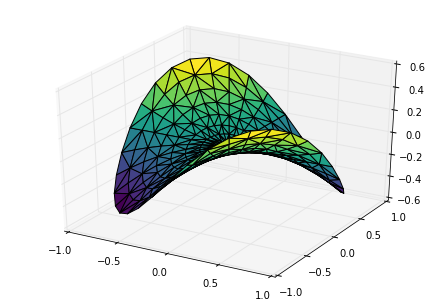
\includegraphics[width=.9\linewidth]{img/plt_8.png}


\subsection{Mayavi}
\label{sec:orgheadline40}

\begin{verbatim}
from numpy import pi, sin, cos, mgrid

dphi, dtheta = pi/250.0, pi/250.0
[phi,theta] = mgrid[0:pi+dphi*1.5:dphi, 0:2*pi+dtheta*1.5:dtheta]
m0 = 4; m1 = 3; m2 = 2; m3 = 3; m4 = 6; m5 = 2; m6 = 6; m7 = 4;

r = sin(m0*phi)**m1 + cos(m2*phi)**m3 + sin(m4*theta)**m5 + cos(m6*theta)**m7
x = r*sin(phi)*cos(theta)
y = r*cos(phi)
z = r*sin(phi)*sin(theta)

# View it.
from mayavi import mlab
s = mlab.mesh(x, y, z)
mlab.savefig('img/plt-maya.png')
print('[[file:img/plt-maya.png]]')
\end{verbatim}

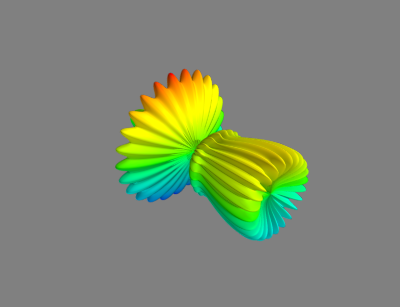
\includegraphics[width=.9\linewidth]{img/plt-maya.png}

\section{OOP}
\label{sec:orgheadline51}

\subsection{O que é OOP?}
\label{sec:orgheadline42}

\begin{enumerate}
\item Programação Orientada Objeto
\item É uma técnica de estruturação do programa
\item Utiliza o conceito de \textbf{Classes} e \textbf{Objetos}
\end{enumerate}

\subsection{Motivação}
\label{sec:orgheadline43}

\begin{verbatim}
# Funcionários (Objeto)
nome1 = 'João'
nome2 = 'Maria'
nome3 = 'Jose'

funcionarios = [nome1, nome2, nome3]

num_funcionarios = len(funcionarios)

# Salario de cada funcionario (Atributo)
salario1 = 10000
salario2 = 12000
salario3 = 8000
\end{verbatim}

\subsection{Como fica em formato de classe?}
\label{sec:orgheadline44}

\begin{verbatim}
class Funcionario():
    'Cria o objeto funcionario'
    contador = 0   # atributo da classe (acessado por todas as instâncias)

    def __init__(self, nome, salario):
        'Método que inicia a classe'
        self.nome = nome
        self.salario = salario
        Funcionario.contador += 1 

    def quantidade(self):
        'Método que mostra o numero de funcionarios'
        print(Funcionario.contador)

func1 = Funcionario('joão', 10000)
func2 = Funcionario('maria', 12000)
print(func1.nome, func1.salario)  # Atributos dos objetos
print(func1.quantidade())       # Invocar um método
\end{verbatim}

\begin{verbatim}
joão 10000
2
\end{verbatim}

\subsection{O que é uma \textbf{Classe}?}
\label{sec:orgheadline45}

\begin{enumerate}
\item É um \uline{construtor} que define um tipo de dado
\item Os dados ficam contidos num container lógico
\item Usar quando houver padrões de comportamento, qualidades e sentido nos dados
\item Contém as \uline{instruções} para criar um \uline{objeto}
\item Permite a definição de \textbf{numenclatura} lógica - facilita a compreensão do código
\end{enumerate}

\begin{verbatim}
class NomeDaClasse():
    'Docstring explica o que a classe cria'

    def __init__(self):
        'Inicia a classe'
        self.atributo = atributo

objeto = NomeDaClasse()
print(objeto.atributo)          # Depois do '.' acesso aos atributos/métodos
\end{verbatim}

\subsection{O que é um \textbf{objeto}, \textbf{método}, \textbf{atributo}?}
\label{sec:orgheadline46}

\begin{enumerate}
\item \textbf{Objeto}
\begin{enumerate}
\item Invocar uma \textbf{classe} significa \uline{instânciar} um \textbf{objeto}
\item Instância: significa "um exemplo", ou  "um caso"
\item As classes definem as características inerentes do objeto
\end{enumerate}
\item \textbf{Atributo}
\begin{enumerate}
\item É uma qualidade do objeto
\item Acessada com '.' \texttt{objeto.atributo}
\end{enumerate}
\item \textbf{Método}
\begin{enumerate}
\item É uma função definida na classe
\item É do objeto
\item Acessada com '.' \texttt{objeto.metodo()}
\end{enumerate}
\end{enumerate}


\subsection{O que é o parâmetro \texttt{self} e o método \texttt{\_\_init\_\_}?}
\label{sec:orgheadline47}

\begin{enumerate}
\item \texttt{self} é a própria instância (objeto) criada pela classe
\item \texttt{\_\_init\_\_} inicializa o objeto
\end{enumerate}
\subsection{Exemplo}
\label{sec:orgheadline48}

\begin{enumerate}
\item Fazer uma classe que contenha instruções para dados de um cachorro
\end{enumerate}

\begin{verbatim}
class Dog():
    'Classe que define o cachorro'
    def __init__(self, name, breed, color):
        self.name = name        # Aplica os atributos
        self.breed = breed
        self.color = color

    def bark(self):
        print('{} barks!!!'.format(self.name))

meu_cachorro = Dog('Euler', 'Poodle', 'Grey')  # Instânciei a classe e criei o objeto

print(meu_cachorro.color)
print(meu_cachorro.bark())
\end{verbatim}

\begin{verbatim}
Grey
Euler barks!!!
None
\end{verbatim}

\subsection{Exercício}
\label{sec:orgheadline49}

Fazer uma classe para uma conta bancária
\subsection{Resultado}
\label{sec:orgheadline50}

\begin{verbatim}
class ContaBancaria:
    def __init__(self):
        self.balanco = 0

    def saque(self, quantia):
        self.balanco -= quantia
        return self.balanco

    def deposito(self, quantia):
        self.balanco += quantia
        return self.balanco

conta_da_maria = ContaBancaria()
conta_do_joao = ContaBancaria()

conta_da_maria.deposito(1000)
print(conta_da_maria.balanco)

conta_da_maria.saque(999)
print(conta_da_maria.balanco)
\end{verbatim}

\begin{verbatim}
1000
1
\end{verbatim}
\end{document}